\documentclass{beamer}
\usepackage{fontspec}
\usepackage{xunicode}
\usepackage{xltxtra}
\usepackage{xecyr}
\usepackage{hyperref}
\setmainfont[Mapping=tex-text]{DejaVu Serif}
\setsansfont[Mapping=tex-text]{DejaVu Sans}
\setmonofont[Mapping=tex-text]{DejaVu Sans Mono}
\usepackage{polyglossia}
\setdefaultlanguage{russian}
\usepackage{graphicx}
\usepackage{listings}
\lstdefinestyle{mycode}{
  belowcaptionskip=1\baselineskip,
  breaklines=true,
  xleftmargin=\parindent,
  showstringspaces=false,
  basicstyle=\footnotesize\ttfamily,
  keywordstyle=\bfseries,
  commentstyle=\itshape\color{gray!40!black},
  stringstyle=\color{red},
  numbers=left,
  numbersep=5pt,
  numberstyle=\tiny\color{gray},
}
\lstset{escapechar=@,style=mycode}
\setbeamerfont{frametitle}{size=\Large}

\begin{document}
\title{Автоматизация анализа популярности технологических областей в корпусе текстов русскоязычных электронных медиа на основе данных Википедии}
%\subtitle{или как всё закодить в декабре, переписать в феврале и поседеть в апреле}
\author{А.М. Алексеев}
\institute{Санкт-Петербургский государственный университет\\математико-механический факультет}

%1. Титульный слайд
% Генерируется автоматичсеки
\frame{\titlepage}

%2. Структура доклада

\begin{frame}\frametitle{Структура доклада}
    \begin{enumerate}
        \item Описание предметной области
        \item Объект автоматизации
        \item Цель и задачи
        \item Данные и выбранный инструментарий
        \item Комплекс программ
        \item Результаты
        \item Формальные признаки
    \end{enumerate}
\end{frame}

%%%3. Описание предметной области и формулировка проблемы, ее актуальность
\begin{frame}\frametitle{Описание предметной области}

\begin{itemize}
\item Web 2.0 как повод для развития Web Science
\item Маркетологические Интернет-исследования на основе текстов на ЕЯ
\item Богатый инструментарий для английского языка
\end{itemize}

\end{frame}
%4. Объект и предмет исследования ЛИБО объект автоматизации (зависит от типа дипломного проекта)
\begin{frame}\frametitle{Объект автоматизации}
Автоматизированное определение того, вместе с какими технологическими областями во влиятельных СМИ в разное время упоминались те или иные организации
\end{frame}

\begin{frame}\frametitle{Цель}
Cоздание комплекса программ, способного установить взаимосвязь упоминаний технологических областей и наименований 
организаций в блогах или новостях на русском языке на основе корпуса текстов 
электронных медиа 
\end{frame}

\begin{frame}\frametitle{Задачи}

\begin{enumerate}
    \item Cбор тестовых данных
    \item Создание комплекса программ, позволяющего 
        \begin{enumerate}
            \item выделять из текста наименования организаций,
            \item выделять из текста технологические области,
            \item строить табличные отчёты по результатам этих двух подзадач,
            \item визуализировать данные отчётов в виде графиков
        \end{enumerate}
\end{enumerate}
\end{frame}

%6. (Подходы к решению, решения, использованный инструментарий)
\begin{frame}\frametitle{Источники данных}

\begin{itemize}
    \item CrunchBase
    \item Habrahabr.ru
    \item Lenta.ru: <<Наука и техника>>
    \item Русскоязычная и англоязычная версии Википедии
\end{itemize}
\end{frame}

\begin{frame}\frametitle{Структура Википедии}
Помимо статей, текстовых ссылок и заголовков, пользователями Википедии поддерживается <<дерево категорий>>

\begin{figure}[ht]
\begin{center}
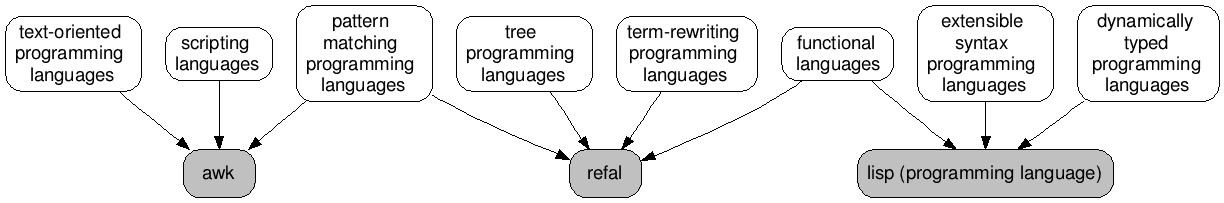
\includegraphics[height=0.75in]{chart_languages.png}
\end{center}
\end{figure}

\begin{figure}[ht]
\begin{center}
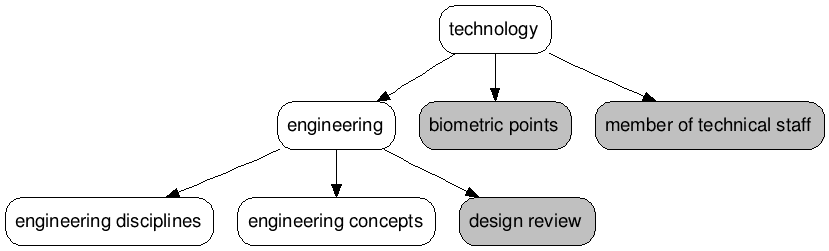
\includegraphics[height=1.2in]{chart_categories.png}
\end{center}
\end{figure}
\end{frame}

\begin{frame}\frametitle{Использованный инструментарий}

\begin{figure}[ht]
\begin{center}
\includegraphics[height=0.5in]{scala.png}
\includegraphics[height=0.5in]{java_logo.jpg}
\includegraphics[height=0.5in]{python.png}
\end{center}
\end{figure}

\begin{figure}[ht]
\begin{center}
\includegraphics[height=0.5in]{maven.png}
\includegraphics[height=0.5in]{apache.png}
\includegraphics[height=0.5in]{lucene.png}
\end{center}
\end{figure}

\begin{itemize}
    \item Scala
    \item Java
    \item Python
    \item WikiXMLJ
    \item russianmorphology
    \item slf4j + logback
    \item Apache Commons
    \item Apache Lucene
    \item Apache Maven
\end{itemize}

\end{frame}


%7. Программный комплекс/программа: состав, архитектура, диаграммы
%классов, структура БД, фуекциональность, результаты работы и пр.
\begin{frame}\frametitle{Комплекс программ: модуль извлечения наименований организаций}
\begin{enumerate}
\item Токенизация
\item Стемминг
\item Поиск подстрок из сформированного списка нормализованных наименований организаций
\end{enumerate}
\end{frame}

\begin{frame}\frametitle{Комплекс программ: модуль извлечения технологических областей~[1]}
\begin{enumerate}
        \item Предобработка
        \begin{enumerate}
		\item ~Токенизация
		\item ~Фильтрация по списку стоп-слов
		\item ~Фильтрация по списку нормализованных слов, встречавшихся в текстах ссылок и заголовков Википедии
        \end{enumerate}
\end{enumerate}
\end{frame}

\begin{frame}\frametitle{Комплекс программ: модуль извлечения технологических областей~[2]}
\begin{enumerate}
         \setcounter{enumi}{2}
        \item Поиск технологических областей
        \begin{enumerate} 
		\item ~Поиск в тексте заголовков русскоязычной Википедии с помощью инвертированного индекса Lucene
		\item ~Переход к англоязычным версиям найденных статей
		\item ~<<Восхождение>> по BFS-дереву категории \textbf{Technology} в графе категорий англоязычной версии Википедии
		 \item ~Запоминание всех посещённых вершин графа как технологических областей
        \end{enumerate}
\end{enumerate}

\end{frame}

\begin{frame}\frametitle{Примеры графиков [1]}
\begin{figure}[ht]
\begin{center}
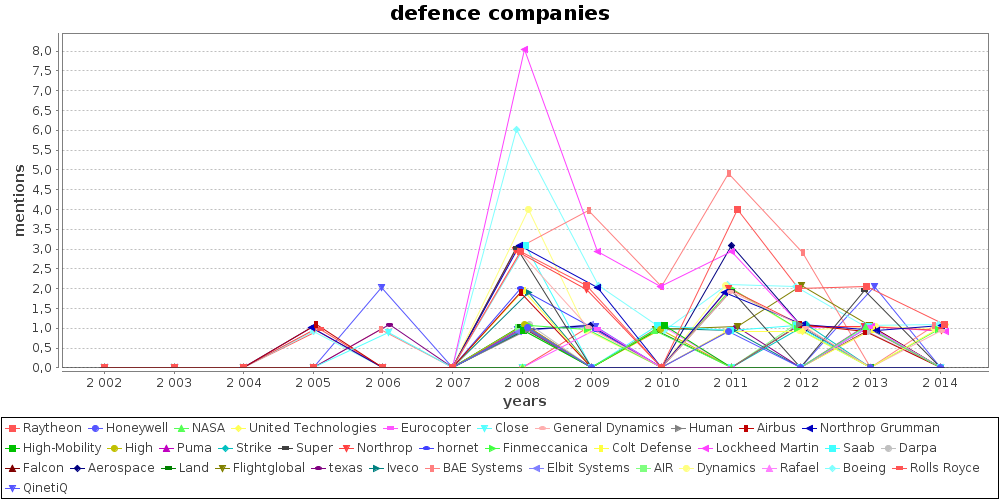
\includegraphics[width=4.5in]{war.png}
\end{center}
\end{figure}
\end{frame}

\begin{frame}\frametitle{Примеры графиков [2]}
\begin{figure}[ht]
\begin{center}
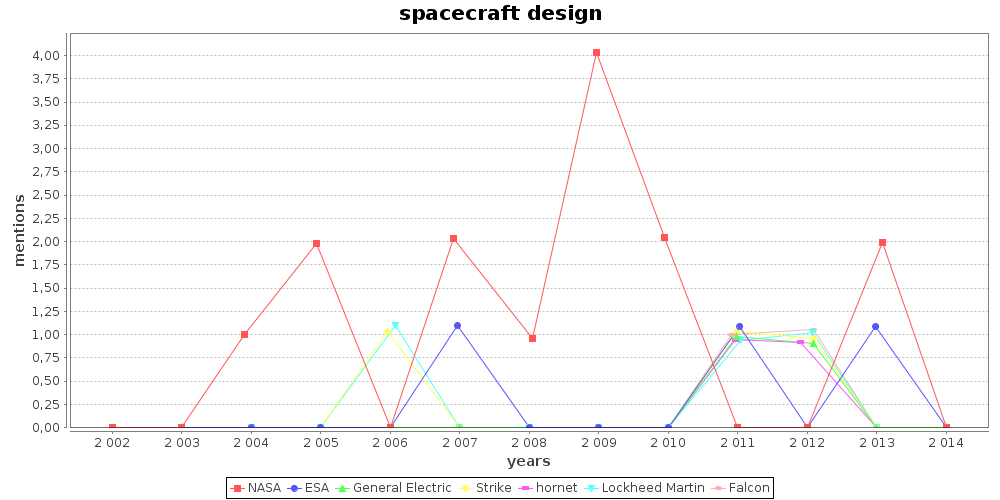
\includegraphics[width=4.5in]{space.png}
\end{center}
\end{figure}
\end{frame}

\begin{frame}\frametitle{Примеры графиков [3]}
\begin{figure}[ht]
\begin{center}
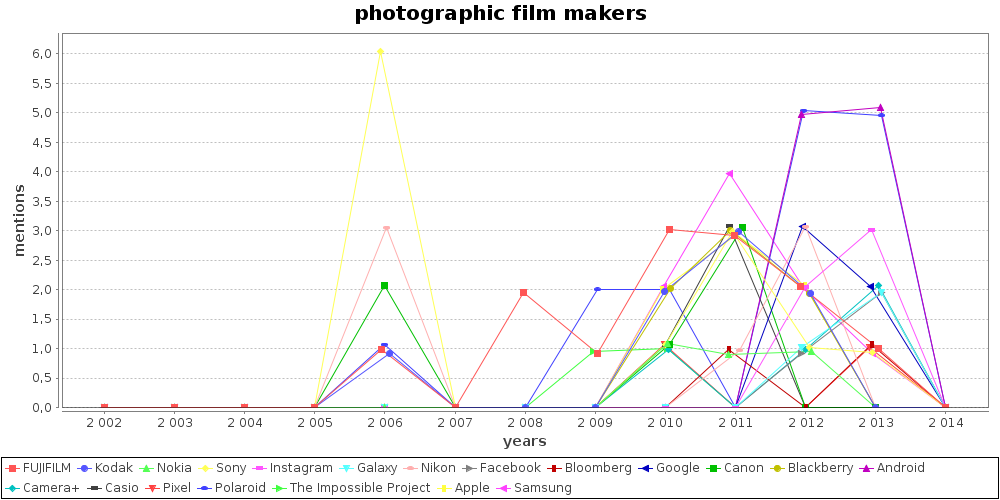
\includegraphics[width=4.5in]{film.png}
\end{center}
\end{figure}
\end{frame}

\begin{frame}\frametitle{Пример графического интерфейса}
\begin{figure}[ht]
\begin{center}
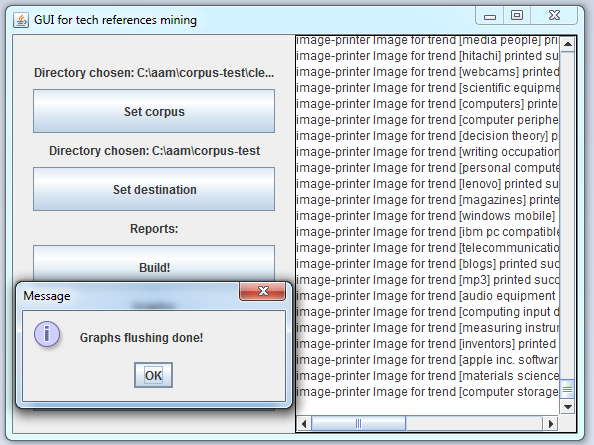
\includegraphics[height=2.5in]{gui.png}
\end{center}
\end{figure}
\end{frame}

%8. Рузультаты
\begin{frame}\frametitle{Результаты}


\begin{enumerate}
    \item Тестовые данные собраны
    \item Созданный комплекс программ  
        \begin{enumerate}
            \item выделяет из текста наименования организаций,
            \item выделяет из текста технологические области,
            \item строит табличные отчёты по результатам этих двух подзадач,
            \item визуализирует данные отчётов в виде графиков
        \end{enumerate}
\end{enumerate}
\end{frame}


%9. "Блестяшки": регистрации, публикации, доклады
% доклад окончен, спасибо за внимание, я готов ответить на Ваши вопросы
\begin{frame}\frametitle{Формальные признаки}
\begin{itemize}
    \item Доклад, подробно описывающий подход, представлен на всероссийской конференции <<СПИСОК-2014>>
    \item Более 5000 строк программного кода на Scala, Java и Python и негенерированного XML
\end{itemize}
\end{frame}

%10. Повтор титульного слайда

\frame{\titlepage}

\end{document}
